\documentclass[]{article}
\usepackage{lmodern}
\usepackage{amssymb,amsmath}
\usepackage{ifxetex,ifluatex}
\usepackage{fixltx2e} % provides \textsubscript
\ifnum 0\ifxetex 1\fi\ifluatex 1\fi=0 % if pdftex
  \usepackage[T1]{fontenc}
  \usepackage[utf8]{inputenc}
\else % if luatex or xelatex
  \ifxetex
    \usepackage{mathspec}
  \else
    \usepackage{fontspec}
  \fi
  \defaultfontfeatures{Ligatures=TeX,Scale=MatchLowercase}
\fi
% use upquote if available, for straight quotes in verbatim environments
\IfFileExists{upquote.sty}{\usepackage{upquote}}{}
% use microtype if available
\IfFileExists{microtype.sty}{%
\usepackage{microtype}
\UseMicrotypeSet[protrusion]{basicmath} % disable protrusion for tt fonts
}{}
\usepackage[margin=1in]{geometry}
\usepackage{hyperref}
\hypersetup{unicode=true,
            pdftitle={Standardization \& Balancing Commodity Tree dataset content and usage in the Food Blance Sheet framework},
            pdfauthor={Cristina Muschitiello~Food and Agriculture Organization of the United Nations},
            pdfkeywords={Commodity Tree, FBS, CPC, shares, extraction Rates, conversion factors},
            pdfborder={0 0 0},
            breaklinks=true}
\urlstyle{same}  % don't use monospace font for urls
\usepackage{longtable,booktabs}
\usepackage{graphicx,grffile}
\makeatletter
\def\maxwidth{\ifdim\Gin@nat@width>\linewidth\linewidth\else\Gin@nat@width\fi}
\def\maxheight{\ifdim\Gin@nat@height>\textheight\textheight\else\Gin@nat@height\fi}
\makeatother
% Scale images if necessary, so that they will not overflow the page
% margins by default, and it is still possible to overwrite the defaults
% using explicit options in \includegraphics[width, height, ...]{}
\setkeys{Gin}{width=\maxwidth,height=\maxheight,keepaspectratio}
\IfFileExists{parskip.sty}{%
\usepackage{parskip}
}{% else
\setlength{\parindent}{0pt}
\setlength{\parskip}{6pt plus 2pt minus 1pt}
}
\setlength{\emergencystretch}{3em}  % prevent overfull lines
\providecommand{\tightlist}{%
  \setlength{\itemsep}{0pt}\setlength{\parskip}{0pt}}
\setcounter{secnumdepth}{5}
% Redefines (sub)paragraphs to behave more like sections
\ifx\paragraph\undefined\else
\let\oldparagraph\paragraph
\renewcommand{\paragraph}[1]{\oldparagraph{#1}\mbox{}}
\fi
\ifx\subparagraph\undefined\else
\let\oldsubparagraph\subparagraph
\renewcommand{\subparagraph}[1]{\oldsubparagraph{#1}\mbox{}}
\fi

%%% Use protect on footnotes to avoid problems with footnotes in titles
\let\rmarkdownfootnote\footnote%
\def\footnote{\protect\rmarkdownfootnote}

%%% Change title format to be more compact
\usepackage{titling}

% Create subtitle command for use in maketitle
\newcommand{\subtitle}[1]{
  \posttitle{
    \begin{center}\large#1\end{center}
    }
}

\setlength{\droptitle}{-2em}
  \title{Standardization \& Balancing\\
\texttt{Commodity\ Tree} dataset\\
content and usage in the Food Blance Sheet framework}
  \pretitle{\vspace{\droptitle}\centering\huge}
  \posttitle{\par}
  \author{Cristina Muschitiello~Food and Agriculture Organization of the United
Nations}
  \preauthor{\centering\large\emph}
  \postauthor{\par}
  \predate{\centering\large\emph}
  \postdate{\par}
  \date{8 June 2018}

\usepackage{lscape}
\usepackage{booktabs}
\usepackage{longtable}
\usepackage{array}
\usepackage{multirow}
\usepackage[table]{xcolor}
\usepackage{wrapfig}
\usepackage{float}
\usepackage{colortbl}
\usepackage{pdflscape}
\usepackage{tabu}
\usepackage{threeparttable}
\usepackage{threeparttablex}
\usepackage[normalem]{ulem}
\usepackage{makecell}

\usepackage{draftwatermark}
\usepackage{makeidx}
\makeindex
\usepackage{float}
\floatplacement{figure}{H}
\usepackage{amsmath}
\usepackage{amssymb}
\usepackage{amsthm}
\usepackage{mathtools}
\usepackage{caption}

\begin{document}
\maketitle
\begin{abstract}
This vignette provides a description of the \texttt{Commodity\ Treee}
dataset: it plays a key role in the Standardization and Balancing and
has been completely renewed in the new Food Balancing Framework. A
description is given in this document, functional to the Standardization
and Balancing Process.
\end{abstract}

{
\setcounter{tocdepth}{4}
\tableofcontents
}
\newpage

\listoftables

\listoffigures

\subsection*{Disclaimer}\label{disclaimer}
\addcontentsline{toc}{subsection}{Disclaimer}

This Working Paper should not be reported as representing the official
view of the FAO. The views expressed in this Working Paper are those of
the author and do not necessarily represent those of the FAO or FAO
policy. Working Papers describe research in progress by the authors and
are published to elicit comments and to further discussion.

This paper is dynamically generated on \today{} and is subject to
changes and updates.

\newpage

\section{Introduction}\label{introduction}

The process of combining commodity balances for creating Food Balance
Sheets is explained in a separate document\footnote{see Standardization
  \& Balancing for Food Balance Sheet Calculation}. The process is based
on a structured and clear set of relationships between commodity given
by the \emph{Commodity tree}. The majority of the commodities are
produced from one (or more) commodity (/ies), called \emph{parent}
commodity(/ies), and/or are themselves parent of one (or more)
\emph{child} (\emph{children}) commodity (/ies). These structure creates
an intense and articulated network of relationships at different levels:
primary commodities, like crops, are \emph{parent} commodities and,
also, \emph{zero-level} commodities from which \emph{children}
commodities of \emph{level-1} are produced, which are in turn, used to
produce other commodities of a gradually \emph{``lower''} level. In
commodity trees, the bigger the level number, the lower the processing
level. There are as many commodity trees as the number of process chains
in a country. The reference document concerning the conversion factors
from parent to processed commodity is available in the documentation
folder on
\href{https://github.com/SWS-Methodology/faoswsStandardization/tree/master/documentation}{\emph{GitHub}}.
The document gives some generic as well as some country specific tcf.
Other details are included in the following document:
\href{https://github.com/SWS-Methodology/faoswsStandardization/blob/master/documentation/flexible_aggregation_of_FAO_supply_utilization_account.pdf}{\emph{Flexible
aggregation of FAO's Supply Utilization Accounts}.}

\section{Content}\label{content}

Commodity trees are presented in tables like Table 1, which represents
the Commodity tree of Wheat in China in the year 2014.

\begin{longtable}[]{@{}rlllll@{}}
\caption{Commodity Tree - China/Wheat/2014}\tabularnewline
\toprule
Country & Year & ParentName & ChildName & eR & share\tabularnewline
\midrule
\endfirsthead
\toprule
Country & Year & ParentName & ChildName & eR & share\tabularnewline
\midrule
\endhead
China, Mainland & 2014 & Wheat & Wheat and meslin flo & 0.78 &
1.00\tabularnewline
China, Mainland & 2014 & Wheat & Bran of Wheat & 0.22 &
1.00\tabularnewline
China, Mainland & 2014 & Wheat and meslin flo & Uncooked pasta, not &
1.00 & 1.00\tabularnewline
China, Mainland & 2014 & Wheat and meslin flo & bread & 1.00 &
1.00\tabularnewline
China, Mainland & 2014 & Wheat and meslin flo & pastry & 1.00 &
1.00\tabularnewline
China, Mainland & 2014 & Wheat and meslin flo & Starch of Wheat & 0.75 &
1.00\tabularnewline
China, Mainland & 2014 & Wheat and meslin flo & Wheat Gluten & 0.08 &
1.00\tabularnewline
China, Mainland & 2014 & Wheat and meslin flo & Communion wafers, em &
1.00 & 1.00\tabularnewline
China, Mainland & 2014 & Starch of Wheat & Other Fructose and S & 1.00 &
1.00\tabularnewline
China, Mainland & 2014 & Wheat Gluten & Gluten Feed and Meal & 1.00 &
0.33\tabularnewline
China, Mainland & 2014 & Bran of Maize & Gluten Feed and Meal & 1.00 &
0.67\tabularnewline
\bottomrule
\end{longtable}

In the table:

\begin{itemize}
\tightlist
\item
  each production process is represented in a separate row.
\item
  \emph{Wheat and meslin flour} and \emph{Bran of wheat} are both
  produced from Wheat.
\item
  From 1 unit of Wheat 0.78 units of Flour is produced and 0.22 units of
  Bran of wheat\footnote{tons is the usual measurement unit for wheat}.
\item
  \emph{Wheat and meslin flour} is produced 100\% from Wheat, as well as
  \emph{Bran of Wheat}. This information is contained in the
  \emph{share} equal to 1.
\item
  From \emph{Wheat and meslin flour} 6 different processed commodities
  are produced (in China). All of them but 2 have an extraction rate
  equal to 1, meaning that 1 unit is produced from each unit of flour.
  \emph{Starch of Wheat} and \emph{Wheat Gluten} have a smaller
  extraction rate instead.
\item
  \emph{Gluten feed and meal} can be produced both from \emph{Wheat
  Gluten} and from \emph{Bran of Maize}\footnote{This commodity pertain
    to the \emph{Maize} commodity tree, but is reported here for
    explaining this Tree}. In particular: in this country 33\% of
  \emph{Gluten feed and meal} comes from \emph{Wheat Gluten} and 67\%
  from \emph{Bran of Maize}.
\end{itemize}

Each production process is, therefore, represented by two main values:
\emph{extraction rate} and \emph{share}.

\subsection{Extraction Rates}\label{extraction-rates}

\textbf{\emph{Extraction rates}} (\(eR\)) represent how much amount of
the child commodity is produced from 1 unit of parent commodity. In the
table they are reported as ratios, other time they can be presented as
percentages. Extraction Rates may differ fro country to country and, in
the same country, from year to year, for example if the country changes
one production process for some commodity. In Commodity Tree tables,
extraction rates may be equal to 0 or NA. In both cases this means that
the production process expressed in the specific line is possible
(i.e.~some other country has or has had it) but for that specific year
in that country it is not active.

Extraction rates are fixed, they are determined once and remains fixed
for the specific year. For following year they might:

\begin{itemize}
\tightlist
\item
  change, if the Country communicate that something has changed in the
  way it produces some specific commodity
\item
  appear, if not existing before, when a country starts producing
  commodities it was not producing in the past
\item
  disappear, if the country deactivates some production process.
\end{itemize}

\subsection{Shares}\label{shares}

Some child commodity can be produced starting from more that one parent
commodity. \textbf{\emph{Shares }} represents the amount of a child
commodity that is produced from each parent commodity. Shares can be
expressed as ratio or percentage.

In the previous Food Balance Sheet Framework shares were given a-priori.
They were given by country and were fixed, as the extraction rates. Each
share represented the amount of a \emph{parent commodity} used for
producing each processed commodity. In other words, shares were
\emph{parent-specified} and given \emph{a-priori}

In the new FBS framework, Shares are \emph{endogenously} calculated
inside the process of standardization. Shares are based on actual
availabilities and are \emph{child-specified}. In general terms,
\emph{shares} are given by:

\begin{equation}
\label{eq:sharesGen}
s_{cp} = \frac{availability_{p(c)}}{\sum \limits_{p=1}^A{availability_{p(c)}}}
\end{equation}

where \(availability_{p(c)}\) is the availability of each parent \(p\)
of child \(c\) expressed in terms of \(c\) (in \emph{child equivalent}).

Shares are calculated twice during the standardization process, using
two different \emph{availabilities.}

\begin{enumerate}
\def\labelenumi{\arabic{enumi}.}
\tightlist
\item
  During Food Processing calculation.
\end{enumerate}

\begin{quote}
Food processing is the amount of the supply of a commodity processed
into derived commodities. Food processing is calculated for all the
parent commodities as the sum of the food processing of all the possible
derived commodities. For its calculation only the amount of each child
that is actually being produced by one parent has to be used. Therefore,
a ratio representing how much of a child has to be back used is given by
the \emph{share} defined as \(s^1_{cp}\):
\end{quote}

\begin{quote}
\begin{equation}
\label{eq:shares}
s^{1}_{cp} = \frac{availability1_{p(c)}}{\sum \limits_{p=1}^A{availability1_{p(c)}}}
\end{equation}
\end{quote}

\begin{quote}
where \(availability1_{p(c)}\) is the availability of each parent \(p\)
of child \(c\) expressed in terms of \(c\) (as say in \emph{child
equivalent}) defined as:
\end{quote}

\begin{quote}
\begin{equation}
\label{eq:availability 1}
availability1_{p(c)} = (P_{pjt} + I_{pjt} - X_{pjt})\times eR_{p\to c}
\end{equation}
\end{quote}

\begin{quote}
where \(P\)=Production, \(I\)=Imports and \(X\)=Exports and where the
\(i\) index runs over all countries, the \(j\) index over all
commodities, and \(t\) over years.
\end{quote}

\begin{quote}
Here, the amount \emph{available} of each parent is represented by a
reduced version of the concept of Total Supply (TS). Indeed
\(TS = P + I - X \pm \Delta S\) (\(\Delta S\) representing changes in
stock). Anyhow here stocks are not used, because the model imputing
stock is considered as needing refinement and the stock figures proved
to create deep fluctuations in results.
\end{quote}

\begin{enumerate}
\def\labelenumi{\arabic{enumi}.}
\setcounter{enumi}{1}
\tightlist
\item
  During Standardization.
\end{enumerate}

\begin{quote}
When the Standardization happens, each commodity is tranformed in its
parent equivalent. A ratio specifying how much of each child has to be
back standardizaed is needed also in this step. This time the amount of
each parent \emph{available} for the processing if the \emph{Food
Processing}, therefore, in the definition of \(s^2_{cp}\) the
availability is the Food Processing (\(FP\)):
\end{quote}

\begin{quote}
\begin{equation}
\label{eq:shares}
s^{2}_{cp} = \cfrac{availability2_{p(c)}}{\sum \limits_{p=1}^A{availability2_{p(c)}}}
\end{equation}
\end{quote}

\begin{quote}
and
\end{quote}

\begin{quote}
\begin{equation}
\label{eq:availability2}
availability2_{p(c)} = FP_{p}\times eR_{p\to c}
\end{equation}
\end{quote}

\section{Representation}\label{representation}

Commodity tree are ofnet visualized and explored in a flowchart frorm of
the kind presented in Figure \ref{fig:f1}. The figure is a screenshot
from the \emph{tcf} document where:

\begin{itemize}
\tightlist
\item
  \textbf{\emph{nodes}} represent commodities,
\item
  \textbf{\emph{edges}} represent production processes ,
\item
  \textbf{\emph{joints}} indicate where a single production process
  creates more that one commodity. These commodities are, then, called
  \emph{by-products} or \emph{co-products}.
\end{itemize}

In the image a \emph{general} commodity tree is presented for Wheat.
Percentages reported are average extraction rates from the parent to the
child commodity. Intervals and average values calculated on all
countries are reported. Moreover, in some cases \(eR\)s are not
reported. Commodity trees in graphic form do NOT exist for all countries
in these document, nor in other documents.

Indeed, not all the countries have the same production processes:
countries have different technologies and primary products
availabilities. Therefore, the commodity trees are not the same across
countries and, sometimes, across years. Nevertheless, specific
country-commodity-year trees do exist. For example, for China Mainland
in 2014, the commodity tree would be the one reported in \ref{fig:f2}
and in Table 1.

\begin{figure}[H]

{\centering 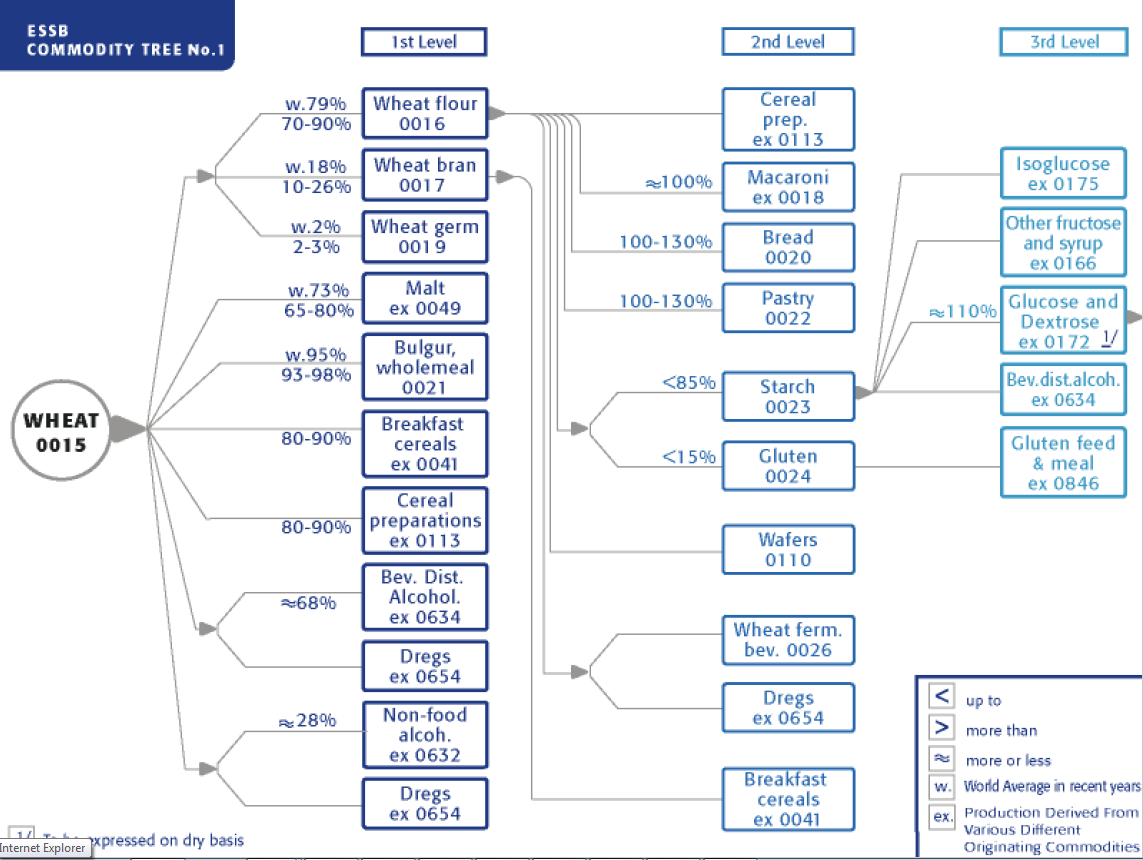
\includegraphics[width=1\linewidth]{images/commodityTree/01_tcfWheat} 

}

\caption{\label{fig:f1}Commodity Tree for Wheat from the tcf document}\label{fig:f1}
\end{figure}

\begin{figure}[H]

{\centering 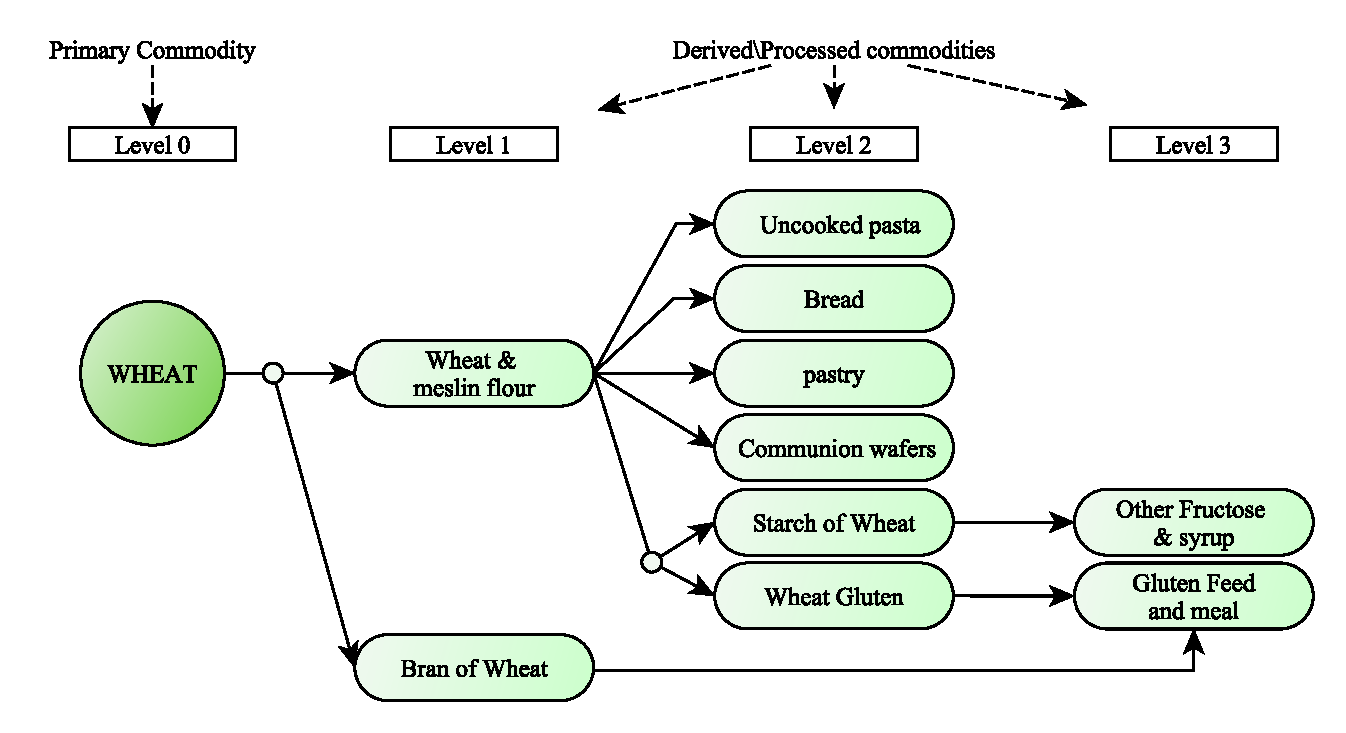
\includegraphics[width=0.9\linewidth]{images/commodityTree/02_WheatTree} 

}

\caption{\label{fig:f2}Commodity Tree China Mainland, Wheat, 2014}\label{fig:f2}
\end{figure}

In the SWS (Statistical Working System of FAO) country-commodity-years
commodity trees are stored in dedicated Data-sets.

\section{Commodity Tree in the SWS}\label{commodity-tree-in-the-sws}

Extraction rates and shares are stored the SWS in the following places.

\begin{enumerate}
\def\labelenumi{\arabic{enumi}.}
\tightlist
\item
  \emph{Shares} from the old FBS system are stored in the
  \texttt{agriculture:aupus\ share} data-set
\end{enumerate}

\begin{quote}
\emph{Shares} in the new framework are always endogenously computed,
therefore these values have never been used in this context.
\end{quote}

\begin{enumerate}
\def\labelenumi{\arabic{enumi}.}
\setcounter{enumi}{1}
\tightlist
\item
  \(eR\) from the old FBS system are stored in the
  \texttt{agriculture:aupus\ ratio} data-set. These ratios were copied
  from the old system and used in the new system.
\end{enumerate}

\begin{quote}
During the implementation and test of the new methodology, it was
realized that the information stored in the mentioned data-set was not
complete. Old data were then analyzed and real etraction rates extracted
and tested. The new values are now stored in another data-set
\end{quote}

\begin{enumerate}
\def\labelenumi{\arabic{enumi}.}
\setcounter{enumi}{2}
\tightlist
\item
  New Extraction Rates are stored in the
  \texttt{SUA/FBS:Commodity\ tree} dataset. These values were obtained
  by extracting old \(eR\) from SUA tables of the old system in the time
  range 2000-2010. These values were applyed in new SUA tables and The
  Foos Balance Sheets obtained were compared with those already
  plublished in the same time-range. When the two FBS time series
  matched, the \(eR\) were considered validated in that time range. Also
  \emph{shares} were tested in this exercise and saved in the data-set.
  However, these shares represent a ``memory'' of the old values, but
  are never used.
\end{enumerate}

\subsection{\texorpdfstring{\texttt{SUA/FBS:Commodity\ tree}
data-set.}{SUA/FBS:Commodity tree data-set.}}\label{suafbscommodity-tree-data-set.}

The \texttt{Commodity\ tree} dataset is in the \texttt{SUA/FBS} domain.
Figures \ref{fig:f3} and figure \ref{fig:f4} reports an example on China
Mainland. When opening a session the following variables have to be
specified:

\begin{itemize}
\tightlist
\item
  Country
\item
  Elements. Here only two elements are available: Extraction rates and
  Shares
\item
  Parent Item
\item
  Child Item
\item
  Time Range
\end{itemize}

\begin{figure}[H]

{\centering 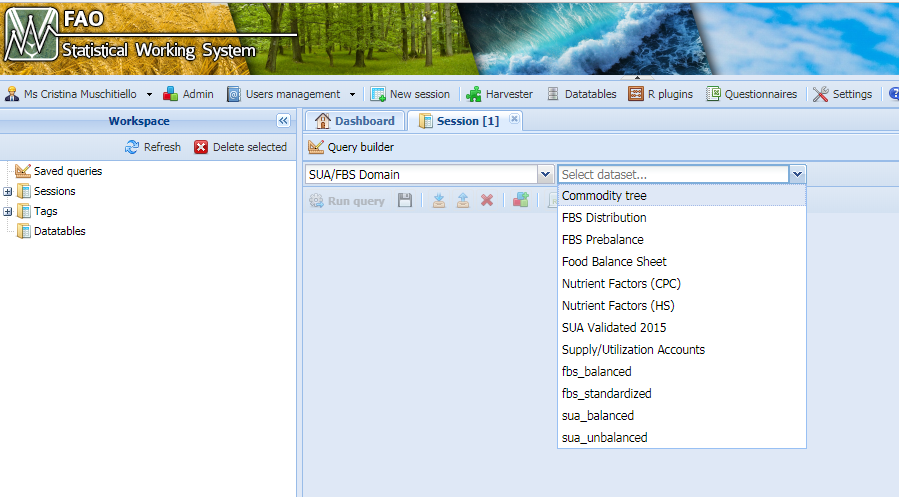
\includegraphics[width=0.9\linewidth]{images/commodityTree/03_selectDataset} 

}

\caption{\label{fig:f3}Selection of the Commodity Treee dataset}\label{fig:f3}
\end{figure}

\begin{figure}[H]

{\centering 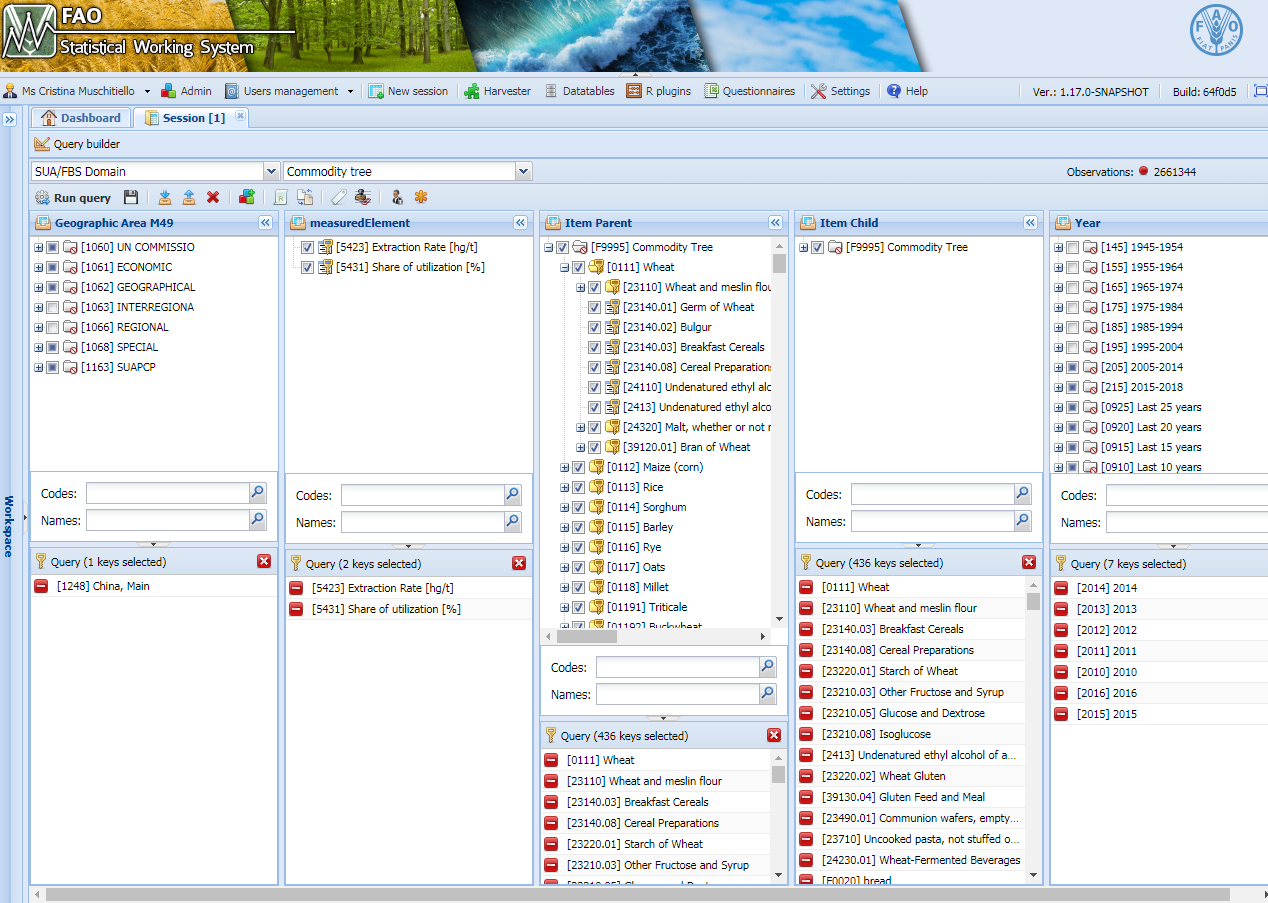
\includegraphics[width=0.9\linewidth]{images/commodityTree/04_selection} 

}

\caption{\label{fig:f4}Selection of parameter in the Commodity Tree - China Mainland example}\label{fig:f4}
\end{figure}

As reported in figure \ref{fig:f5} commodity are listed by country and
for each country:commodity the two variables are displayed.

\begin{figure}[H]

{\centering 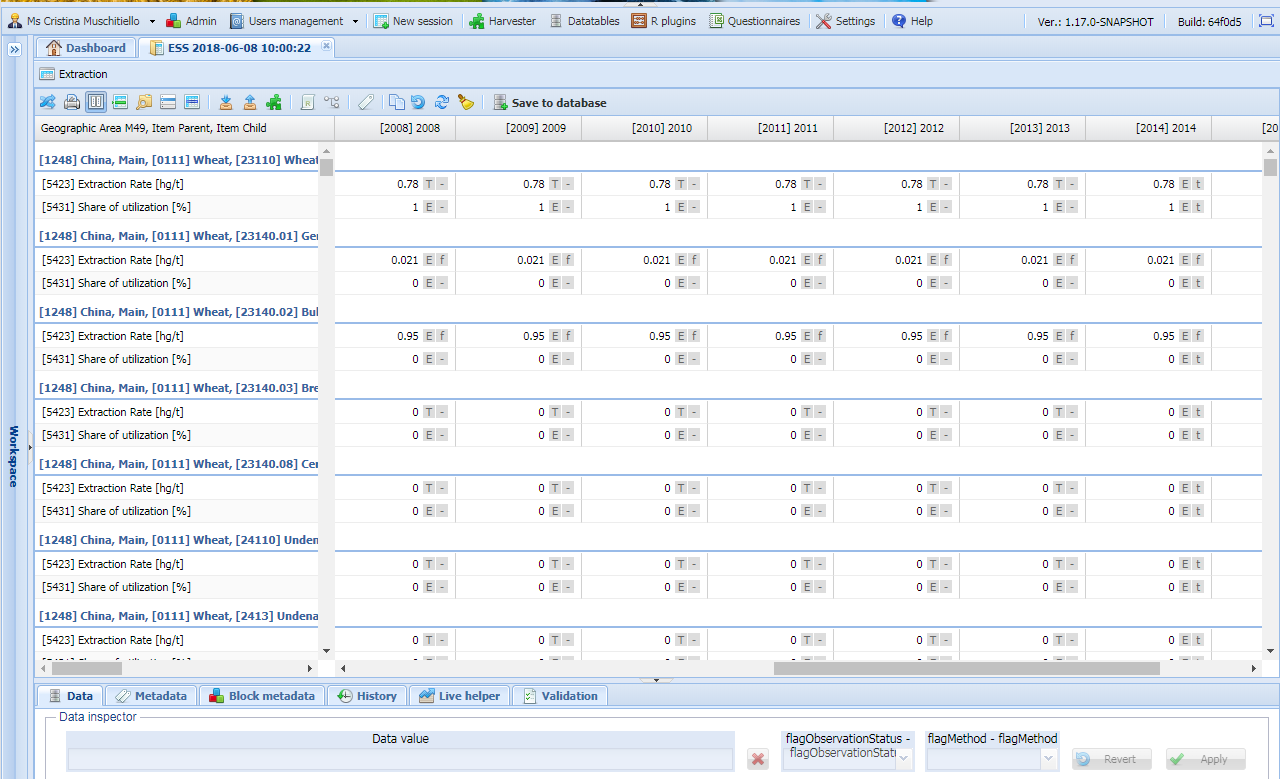
\includegraphics[width=0.9\linewidth]{images/commodityTree/05_session} 

}

\caption{\label{fig:f5}Commodity Tree session - China Mainland example}\label{fig:f5}
\end{figure}

The dtaset contains:

\begin{enumerate}
\def\labelenumi{\arabic{enumi}.}
\tightlist
\item
  \textbf{\emph{Extraction rates}}:
\end{enumerate}

\begin{itemize}
\tightlist
\item
  Extraction rates 2000-2013: these \(eR\) are taken from the old
  framework. These Extraction rates have been validated in this time
  window (2000-2013).
\item
  Extraction rates from 2014 onwards: From 2014 onwards Extraction rates
  of 2013 have been copied.
\end{itemize}

\begin{quote}
Extraction rates are not modified during the standardization process.
They can be manually changed. When this happens, manually inserted
figures are considered protected and preferred over the others.
\end{quote}

\begin{enumerate}
\def\labelenumi{\arabic{enumi}.}
\setcounter{enumi}{1}
\tightlist
\item
  \textbf{\emph{Shares}}:
\end{enumerate}

\begin{itemize}
\tightlist
\item
  Shares 2000-2013: these shares are taken from the old framework. These
  shares have been validated in this time window (2000-2013).
\item
  Shares from 2014 onwards: From 2014 onwards shares of 2013 have been
  copied.
\end{itemize}

\begin{quote}
Shares are recalculated at each module run. An exception is represented
by \textbf{shares of oils}. Because oils hystorically have had problems,
shares for these commodities is not recalculated but old shares are
used. Shares can also been manually modified. When it happens, the
manual value is used instead, but only after a check is performed on the
consistency of the value.
\end{quote}

\newpage

\subsection{Flag combinations and
interpretation}\label{flag-combinations-and-interpretation}

Different flags are used for identify the tipology of value in the
dataset. The following flags and meanings have been agreed:

\begin{table}[h]
\caption {Flag combination in the Commodity tree data-set}
\centering
\begin{tabular}{|l|l|l|}
\toprule
\bf{Variable} & \bf{Flag Combination} & \bf{Meaning}\\ 
\midrule
\multirow{4}{*}{Extraction Rate} & $(T , -)$  & validated up do 2013 - protected \\
\cline{2-3}
& \multirow{2}{*}{$(E , t)$}  &   copied from 2014 onwards - NOT protected \\
& &  (do not change during standardization process)\\ 
\cline{2-3}
& $(E , f)$  &   manually changed by the user – protected\\ 
\cline{1-3}
\multirow{5}{*}{Share} & \multirow{3}{*}{$(E , -)$}  & coming from old methodology - NOT protected.\\
& &  (overwritten at any run of the module, except the values of oils\\
& &   which are kept, unless manually changed) \\
\cline{2-3}
& $(E , f)$  &  manually changed by the user - protected\\ 
\cline{2-3}
& $(I , i)$  &   calculated by the module - not protected\\ 
\cline{1-3}
\end{tabular}
\end{table}

\subsection{Validity check functions}\label{validity-check-functions}

Because \texttt{Commodity\ tree} data-set is already used in more that 1
module and because in the future it might be used for other purposes, 3
validity fuctions have been created. These functions are included in the
\href{https://sdlc.fao.org/bitbucket/projects/SWS/repos/faoswsutil/browse/R}{\emph{faoswsUtil}
package}.

\subsubsection{\texorpdfstring{\texttt{validateTreeExtractionRates.R}}{validateTreeExtractionRates.R}}\label{validatetreeextractionrates.r}

This function performs 2 checks:

\begin{enumerate}
\def\labelenumi{\arabic{enumi}.}
\tightlist
\item
  if the values are outside a reasonable range that can be manually set
  and that, by default is 0-10
\item
  If the flags are outside those listed in Table 2
\end{enumerate}

it just returns a list of the invalid rows (if any) and a message.

\subsubsection{\texorpdfstring{\texttt{validateTreeShares.R}}{validateTreeShares.R}}\label{validatetreeshares.r}

This function performs 2 checks:

\begin{enumerate}
\def\labelenumi{\arabic{enumi}.}
\tightlist
\item
  if the values are outside the range 0-1
\item
  If the flags are outside those listed in Table 2
\end{enumerate}

it just returns a list of the invalid rows (if any) and a message.

\subsubsection{\texorpdfstring{\texttt{validateTree.R}}{validateTree.R}}\label{validatetree.r}

This function aggregates the validation of shares and Trees and sends
emails containing a message saying that Extraction rates and/or shares
are ok or, if anything is not correct, a csv file containing the wrong
lines.


\end{document}
